\documentclass[11pt]{article}
\usepackage{amsmath,amssymb,amsthm}
\usepackage{graphicx}
\usepackage[margin=1in]{geometry}
\usepackage{fancyhdr}
\usepackage{float}
\setlength{\parindent}{0pt}
\setlength{\parskip}{5pt plus 1pt}
\setlength{\headheight}{13.6pt}
\newcommand\question[2]{\vspace{.25in}\hrule\textbf{#1: #2}\vspace{.5em}\hrule\vspace{.10in}}
\renewcommand\part[1]{\vspace{.10in}\textbf{(#1)}}
\newcommand\algorithm{\vspace{.10in}\textbf{Algorithm: }}
\newcommand\result{\vspace{.10in}\textbf{Result: }}
\pagestyle{fancyplain}
\lhead{\textbf{\NAME\ (\ANDREWID)}}
\chead{\textbf{Assignment\HWNUM}}
\rhead{STAT3006: Statistical Computing}
\begin{document}\raggedright
%Section A==============Change the values below to match your information==================
\newcommand\NAME{ZHANG Xinfang}  % your name
\newcommand\ANDREWID{1155141566}     % your student id
\newcommand\HWNUM{4}              % the homework number
%Section B==============Put your answers to the questions below here=======================

\question{1}{Parallel Computing for EM Alogorithm (40\%)} 

\question{2}{Database Access from R (30\%)}
SQL in the pictures following highlighted in blue in the double quotes.

(a) The 'Book' Table:
\begin{figure}[H]
    \centering
    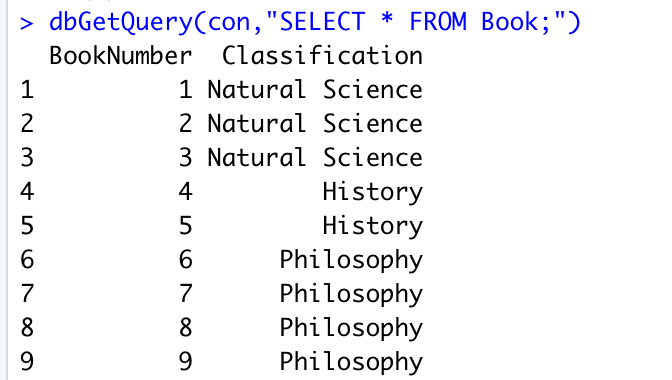
\includegraphics[width=0.4\textwidth]{figures/Q2.1.png}
    \caption{'Book' Tbale}
\end{figure}
(b) 
\begin{figure}[H]
    \centering
    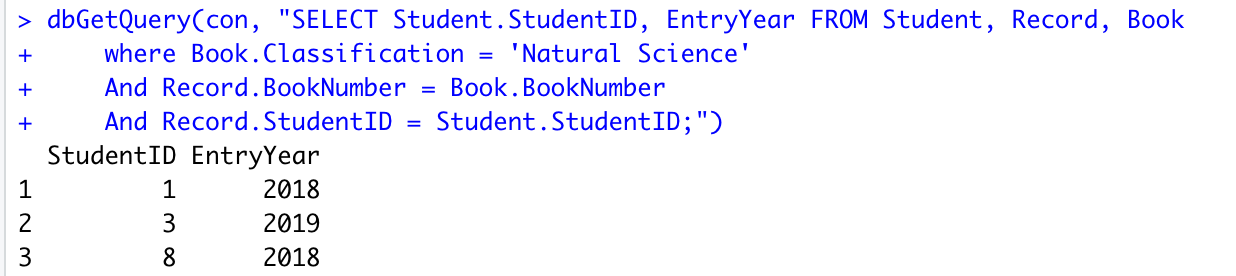
\includegraphics[width=0.7\textwidth]{figures/Q2.2.png}
    \caption{Students who borrowed natural science books}
\end{figure}
(c)
\begin{figure}[H]
    \centering
    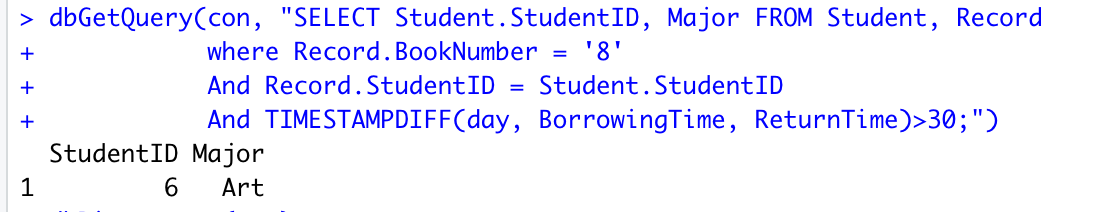
\includegraphics[width=0.7\textwidth]{figures/Q2.3.png}
    \caption{Students who borrowed book 8 for more than 30 days}
\end{figure}

\question{3}{XML (eXtensive Markup Language) (30\%)}



\end{document}